\chapter{Censo Demográfico 2022 - Religiões}
\label{apendice:censo_demografico_2022}

Proporção da população de 10 anos ou mais de idade residente em domicílios particulares permanentes com conexão domiciliar à internet, segundo grandes grupos de religião – 2022.
\begin{figure}[H]
\centering
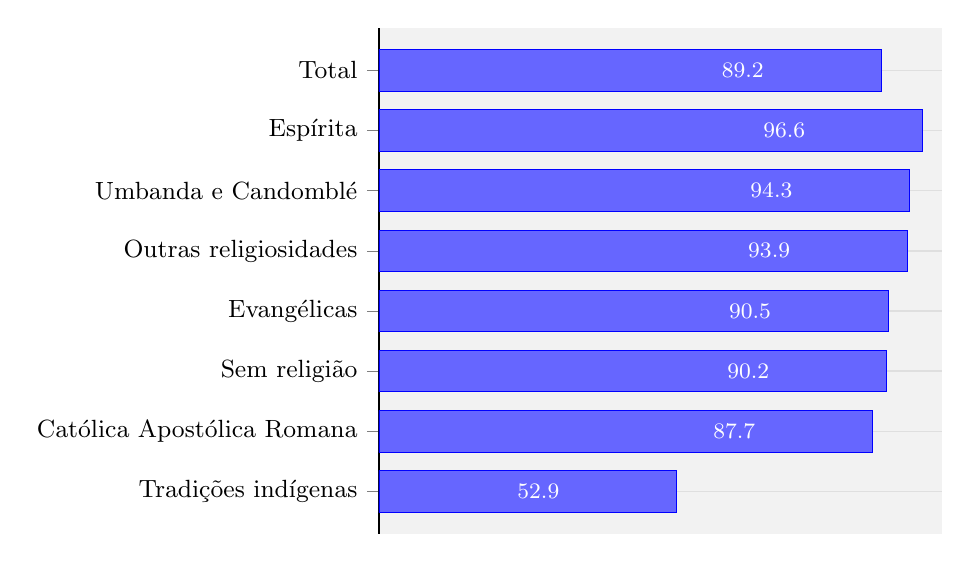
\begin{tikzpicture}
\begin{axis}[
    xbar,
    xmin=0,
    xmax=100,
    width=0.72\textwidth, % Aumentar um pouco a largura do gráfico
    height=8cm,
    xlabel={\% de domicílios com internet},
    symbolic y coords={
        Tradições indígenas,
        Católica Apostólica Romana,
        Sem religião,
        Evangélicas,
        Outras religiosidades,
        Umbanda e Candomblé,
        Espírita,
        Total
    },
    ytick=data,
    nodes near coords,
    nodes near coords align=center, % Alinha os números centralizados nas barras
    every node near coord/.append style={
        font=\footnotesize,
        xshift=-50pt,
        color=white
    }, % Remover o deslocamento
    bar width=15pt, % Aumentando a largura das barras
    % title={Acesso domiciliar à internet por grupo religioso (Censo 2022)},
    tick label style={font=\small},
    label style={font=\small},
    title style={font=\small\bfseries, align=center},
    axis x line=none, % Remover linha do eixo X
    axis y line* = left, % Manter a linha do eixo Y à esquerda
    axis background/.style={fill=gray!10}, % Fundo suave para o gráfico
    grid=both, % Adiciona grid para facilitar a leitura
    grid style={line width=0.2mm, draw=gray!25}, % Estilo da grid
]
\addplot+[
    xbar,
    fill=blue!60,
    mark options={fill=blue!60}
] coordinates {
    (52.9,Tradições indígenas)
    (87.7,Católica Apostólica Romana)
    (89.2,Total)
    (90.2,Sem religião)
    (90.5,Evangélicas)
    (93.9,Outras religiosidades)
    (94.3,Umbanda e Candomblé)
    (96.6,Espírita)
};
\end{axis}
\end{tikzpicture}
\caption{Conexão domiciliar à internet por grupo religioso no Brasil, Censo Demográfico 2022.}
\label{fig:censo_demografico_2022}
% Adicionando as notas abaixo do gráfico
\footnotesize % Ajusta o tamanho da fonte
\begin{flushleft}
    \textbf{Fonte:} Censo Demográfico 2022 \cite{ibge2025religiao}. Dados dos resultados preliminares da amostra, estimados a partir de áreas de ponderação preliminares.\\
    \textbf{Notas}:\\
    1. A categoria Total de ``religião'' inclui as pessoas sem declaração de religião e as que não sabem;\\
    2. A categoria Umbanda e Candomblé de ``religião'' inclui outras religiões afro-brasileiras.
\end{flushleft}
\end{figure}